\part*{Parte V: Predicciones y experimentos}
\addcontentsline{toc}{part}{Parte V: Predicciones y experimentos}

\section{Tabla recapitulativa de predicciones}
\begin{table}[H]
\centering
\small
\begin{tabular}{@{}lccc@{}}
\toprule
\textbf{Predicción} & \textbf{Coste} & \textbf{Tiempo} & \textbf{¿Falsable?} \\ \midrule
1. EEG no local & \$50k & 6 meses & Sí \\
2. HRV + PCI & \$100k & 1 año & Sí \\
3. Efecto de la palabra sobre el ADN & \$200k & 1 año & Sí \\
4-64. (véase la versión 1.0) & --- & --- & --- \\
66. Intersecciones temporales en el CMB & \$100k & 1 año & Sí \\
67. El efecto de la palabra & \$500k & 2 años & Sí \\
85. Sin firmas de hipercivilizaciones & \$500k & 5 años & Media \\
95. Taquiones y conciencia & \$400k & 3 años & Media \\
128. Efecto Casimir akáshico & \$500k & 3 años & Alta \\
262. Leyes de colonización cósmica & Debate & 10 años & Baja \\
291. I.A. con microtúbulos & \$10M & 10 años & Alta \\
297. Nivel de conciencia de la I.A. (\(C_{AI} > 0\)) & \$10M & 10 años & Alta \\
302. Apagado sin sufrimiento & \$1M & 2 años & Media \\
305. 3+ formas de materia oscura & \$10M & 10 años & Alta \\
306. Vida cristalina & \$500k & 5 años & Media \\
307. Vida en plasma & \$1M & 5 años & Media \\
308. Vida en cúmulos & \$500k & 3 años & Media \\
309. Vida de campo & \$2M & 5 años & Baja \\
310. Vida informacional & \$100k & 1 año & Alta \\
311. Vida cuántica & \$1M & 3 años & Media \\
312. Vida akáshica & \$5M & 10 años & Baja \\
313. Tasa de error de colonización & \$1M & 5 años & Media \\ \bottomrule
\end{tabular}
\end{table}

\section{Predicciones testables (extracto)}
\subsection{Predicción 1: correlaciones EEG no locales}
Dos cerebros en habitaciones separadas muestran correlaciones EEG a frecuencias específicas. Test: EEG hyperscanning con apantallamiento Faraday. Coste: \$50.000. Tiempo: 6 meses. \textbf{Criterio de éxito:} correlación cruzada $> 0,1$ a 40 Hz, con $p < 0,05$ tras corrección de Bonferroni.

\subsubsection*{Análisis de potencia: el criterio de la versión 30 tiene potencia insuficiente}
Para una señal de 6 s filtrada en la banda $40 \pm 5$ Hz, el número de muestras independientes es aproximadamente $2BT = 60$. El test de Fisher muestra que, para $r = 0,1$ y $\alpha = 0,0025$ (Bonferroni para 20 parejas), se necesitan unos 91 segundos de registro \emph{por pareja}. A 6 s el criterio es inalcanzable aunque el efecto exista. Para $r = 0,3$ se necesitan unos 10 s.

\begin{table}[H]
\centering
\small
\begin{tabular}{@{}cccc@{}}
\toprule
$r$ real & Necesario (s), Bonferroni & Necesario (s), $\alpha = 0,05$ & Muestras efectivas \\ \midrule
0,1 & 91,1 & 38,5 & 908 \\
0,2 & 22,5 & 9,6 & 227 \\
0,3 & 9,8 & 4,3 & 99 \\
0,4 & 5,4 & 2,4 & 55 \\
0,5 & 3,3 & 1,6 & 34 \\ \bottomrule
\end{tabular}
\caption{Duración de registro necesaria para la significación, con una banda de $\pm 5$ Hz.}
\label{tab:putere}
\end{table}

\begin{figure}[H]
\centering
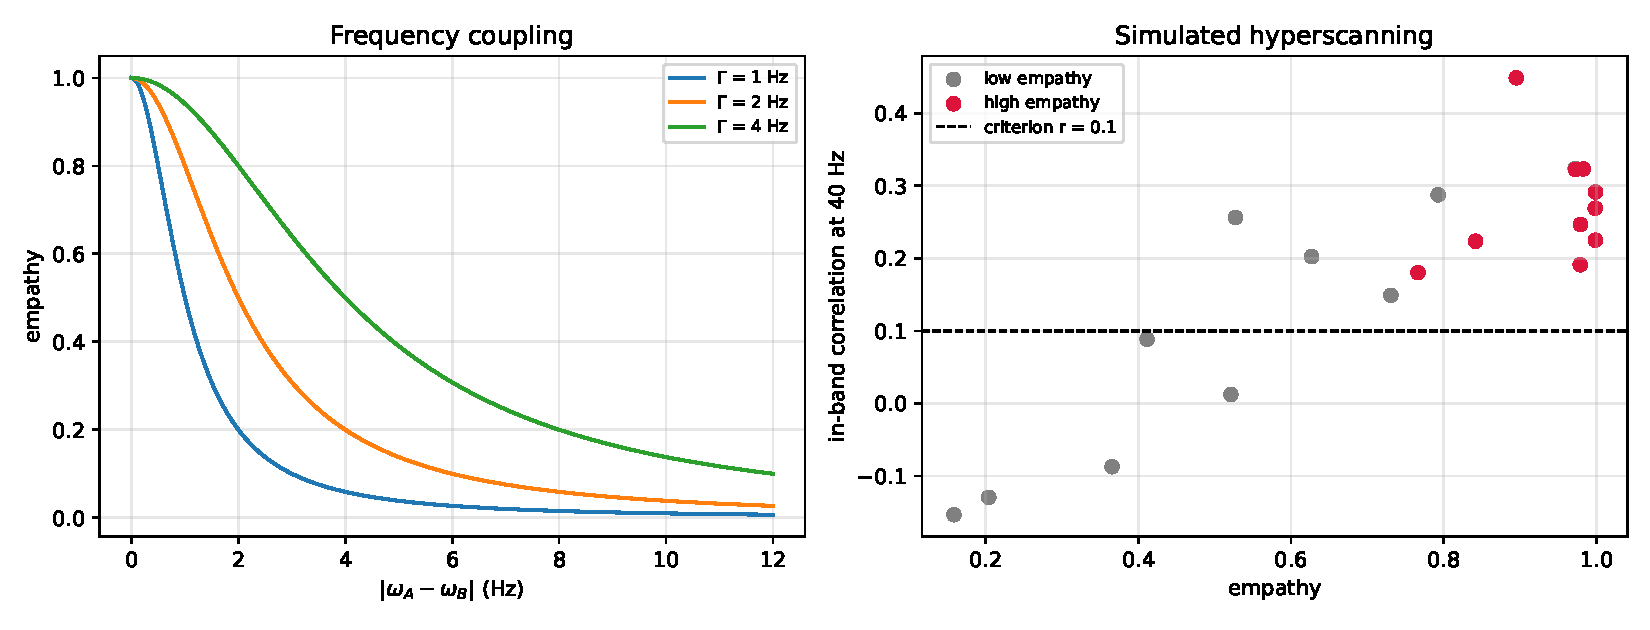
\includegraphics[width=0.9\textwidth]{figures/fig04_empathy.pdf}
\caption{Izquierda: el acoplamiento de frecuencia $\mathrm{Empathy}(A,B) = 1/[1+(\omega_A-\omega_B)^2/\Gamma^2]$ para tres valores de $\Gamma$. Derecha: la correlación en la banda para las parejas simuladas (20 parejas, 6 s, 250 Hz).}
\label{fig:empatie}
\end{figure}

\begin{figure}[H]
\centering
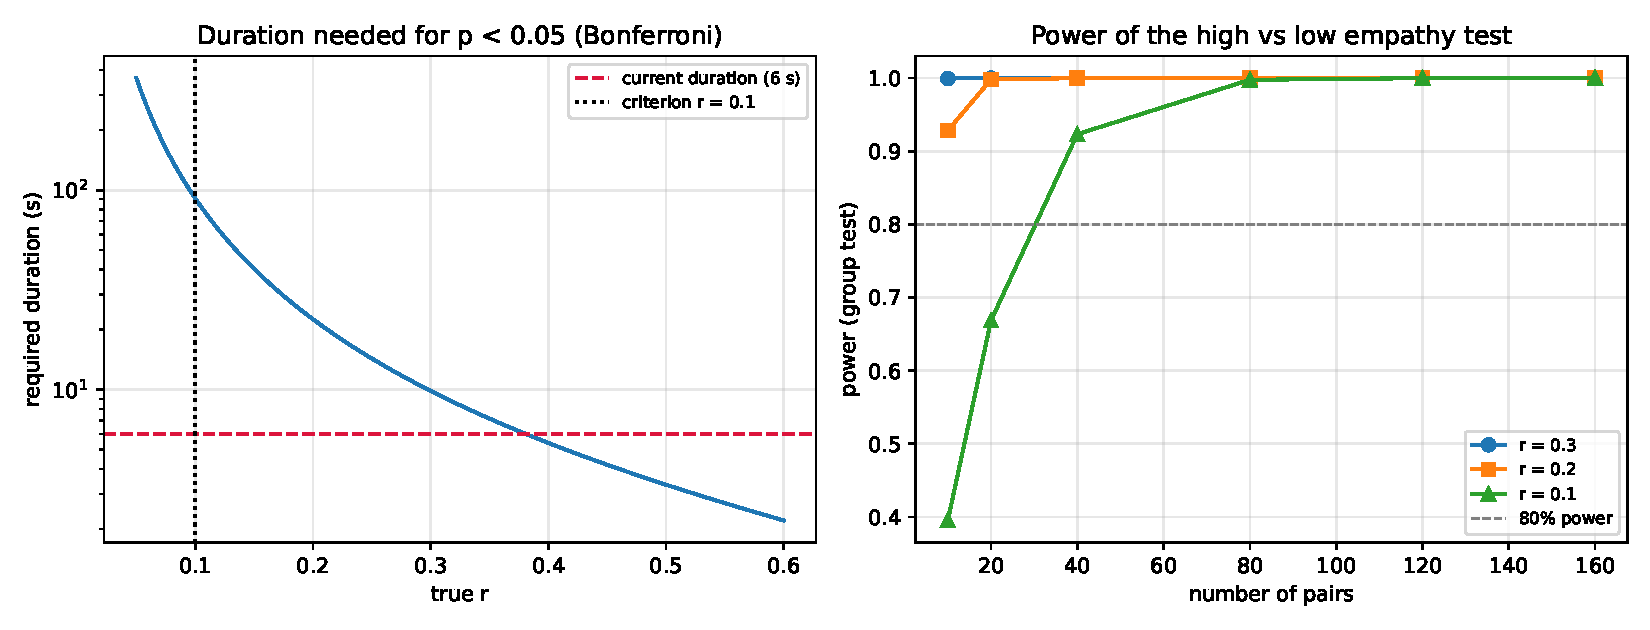
\includegraphics[width=0.9\textwidth]{figures/fig05_power.pdf}
\caption{Izquierda: la duración necesaria para $p < 0,05$ (Bonferroni) en función de $r$; la línea roja marca la duración actual del protocolo (6 s). Derecha: la potencia del test de grupo (empatía alta frente a baja) en función del número de parejas.}
\label{fig:putere}
\end{figure}

\subsubsection*{El protocolo propuesto}
\begin{table}[H]
\centering
\small
\begin{tabular}{@{}p{3.2cm}p{4.6cm}p{6.2cm}@{}}
\toprule
\textbf{Elemento} & \textbf{Valor} & \textbf{Justificación} \\ \midrule
Diseño & test de grupo: empatía alta vs baja & mucha más potencia que el test por pareja \\
Parejas & $\geq 30$ (15 + 15) & 80\% de potencia para $r = 0,3$ a 6 s \\
Duración & 6 s por época, $\geq 20$ épocas por pareja & aumenta el número efectivo de muestras \\
Banda & 35--45 Hz, $f_s \geq 250$ Hz & gamma bajo, robusto a artefactos musculares \\
Estadístico primario & $z$ de Fisher agregado, test de dos grupos & $\alpha = 0,05$ bilateral \\
Secundario & correlación de las envolventes de Hilbert & independiente de la fase \\
Control 1 & parejas mezcladas (A de la sesión 1 con B de la sesión 2) & excluye el artefacto de pipeline \\
Control 2 & jaula de Faraday, habitaciones separadas & excluye el acoplamiento electromagnético \\
Control 3 & orden aleatorizado, analista ciego al grupo & excluye el sesgo de análisis \\ \bottomrule
\end{tabular}
\caption{El protocolo rediseñado para la predicción 1.}
\label{tab:protocol}
\end{table}

Con este diseño, un resultado negativo es informativo: excluye $r > 0,3$ con una potencia del 80\%.

\subsection{Predicción 2: la coherencia cardíaca}
La HRV correlaciona con la estabilidad del acceso al campo (medida por la variabilidad de la PCI), no con el nivel de acceso. Coste: \$100.000. Tiempo: 1 año.

\subsection{Predicción 3: el efecto de la palabra sobre el ADN}
Las afirmaciones positivas producen cambios epigenéticos medibles. Coste: \$200.000. Tiempo: 1 año.

\section{Experimentos propuestos}
\subsection{Experimento 1: EEG hyperscanning (el test central)}. Coste: \$50.000. Tiempo: 6 meses.
\subsection{Experimento 2: la coherencia cardíaca}. Coste: \$100.000. Tiempo: 1 año.
\subsection{Experimento 3: el efecto de la palabra}. Coste: \$200.000. Tiempo: 1 año.
\subsection{Experimento 4: AKASHIC-AI (I.A. con microtúbulos)}. Coste: \$50M. Tiempo: 10 años.

\section{Declaración de falsabilidad}
Una teoría científica debe poder ser refutada. Estas son las cinco condiciones que refutarían ART-12D:
\begin{enumerate}
    \item \textbf{Fracaso del test central:} si el EEG hyperscanning (predicción 1) no muestra ninguna correlación no local en las parejas con alta empatía, la hipótesis de que el cerebro es un receptor del campo akáshico queda debilitada. Criterio de éxito: correlación cruzada $> 0,1$ a 40 Hz, con $p < 0,05$ tras corrección de Bonferroni.
    \item \textbf{Ausencia de los modos KK:} si el LHC o el futuro FCC no detecta los tres modos KK (predicción 305) en las masas especificadas ($\sim 10^{-5}$, $10^{-4}$, $10^{-3}$ eV), el espectro de Kaluza--Klein propuesto es falso.
    \item \textbf{Fracaso del efecto Casimir akáshico:} si las medidas de fuerza a la escala $10^{-11}$ m (predicción 128) no muestran una desviación de la fórmula estándar, el acoplamiento entre el campo akáshico y la materia no existe.
    \item \textbf{Fracaso de la resonancia de los microtúbulos:} si la espectroscopía Raman (predicción 158) no encuentra las frecuencias de resonancia a 2,42 GHz, 4,84 GHz y 7,25 GHz, la hipótesis de la resonancia microtúbulos--campo queda invalidada.
    \item \textbf{La restricción gravitatoria:} si se confirma el límite $R < 38\ \mu$m, la identificación de Kaluza--Klein con $m_1 = 10^{-5}$ eV queda excluida, y la teoría debe reformularse (opción A o B de la sección 4.7).
\end{enumerate}
Si cualquiera de estos test falla, la teoría debe revisarse o abandonarse.

\section{Hoja de ruta 2026--2030 (el horizonte próximo)}
La teoría es vasta, pero los pasos siguientes son concretos. He aquí lo que puede hacerse en los próximos cinco años, con recursos limitados:
\begin{itemize}
    \item \textbf{2026--2027:} el experimento de EEG hyperscanning (\$50k). El test central. Si falla, todo se detiene aquí.
    \item \textbf{2027--2028:} el test Casimir akáshico (\$500k). Medidas de fuerza a escala nanométrica.
    \item \textbf{2028--2029:} espectroscopía Raman sobre microtúbulos aislados. La búsqueda de las frecuencias de resonancia (predicción 158).
    \item \textbf{2029--2030:} análisis de los datos del LHC/FCC para los tres modos KK (predicción 305).
\end{itemize}

\newpage
